\documentclass{homework}

\usepackage{mytoolbox}

\input{particulars}

\renewcommand\thesection{\arabic{section}}
\renewcommand\thesubsection{\arabic{section}.\arabic{subsection}}
\renewcommand\thesubsubsection{\arabic{section}.\arabic{subsection}.\arabic{subsubsection}}

\begin{document}

\title{Deep Learning Lab1}
\author{\chineseName \masterStudentID}
\date{}
\maketitle

\section{Introduction}

In this lab, I implemented a simple neural network with two hidden layers using numpy with backpropagation and training script. The neural network can perform binary classification. 

\section{Implementation Details}

I use Jupyter to run the experiment. At the start, I imported numpy and matplotlib, define the data generation function.

\subsection{Sigmoid function}

For the sigomid function, I used the following formula:

\[
    \sigma(x) = \frac{1}{1 + e^{-x}}
\]

and its derivative is:

\[
    \sigma'(x) = \sigma(x) \cdot (1 - \sigma(x))
\]

with the following implementation:

\begin{lstlisting}[language=Python]
def sigmoid(x):
    return 1.0 / (1.0 + np.exp(-x))

def derivative_sigmoid(x):
    # here x is the sigmoid of another value
    return np.multiply(x, 1.0 - x)
\end{lstlisting}

\subsection{Neural network architecture}

I implemented a neural network model, which can be initialized with a list of layer sizes, allowing for flexible experimentation. So we can create a model as follows:

\begin{lstlisting}[language=Python]
# 4 layers with 2 input, 4 hidden, 4 hidden, 1 output
model1 = Model([2, 4, 4, 1])
\end{lstlisting}

Each layer has a \bfr{weight matrix} and a \bfr{bias vector}. Those are initialized with random values using \lstinline{np.random.randn()}. The forward pass will calculate the activation of each layer using the sigmoid function.

For linearly separable data and XOR data, I both use the same layer sizes [2, 4, 4, 1].

\subsection{Backpropagation}

The backpropagation algorithm is implemented in the \lstinline{backward} method of the model. I tried \bfr{mean squared error} and \bfr{cross-entropy} to calculate the loss. The backpropagation will first calculate the gradient of the loss w.r.t. the output of the last layer, then apply the chain rule to calculate the gradient of \bfr{activation, weight, and bias} of each layer, and update the weights and biases using the gradients times the \bfr{learning rate}.

\subsection{Training}

The training script is implemented in the \lstinline{train} method. It will run the forward and backward pass for each epoch. I also implemented \bfr{early stopping} with \lstinline{patience} parameter. The training will stop if the loss does not decrease for \lstinline{patience} epochs.

For linearly separable data, I use lr=100. For XOR data, I use lr=1.

\section{Experimental Results}

\subsection{Screenshot and comparison figure}

\subsubsection{Linearly separable data}

Training loss and testing prediction:

\begin{figure}[H]
    \centering
    \begin{subfigure}{0.45\textwidth}
        \centering
        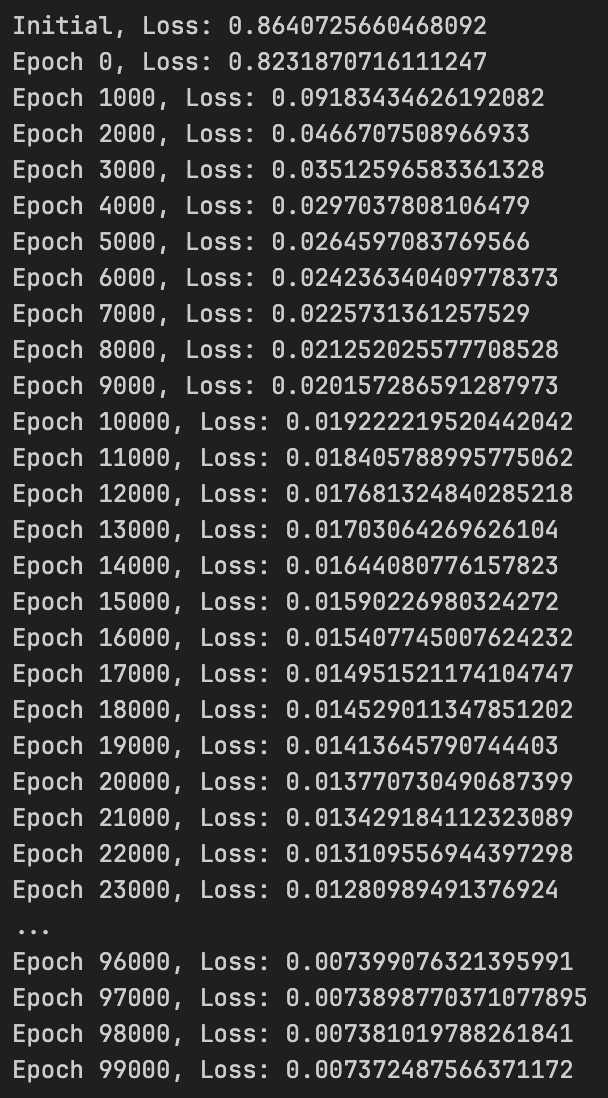
\includegraphics[width=0.6\textwidth]{linear_train.png}
        \caption{Linearly separable data training loss}
    \end{subfigure}
    \begin{subfigure}{0.45\textwidth}
        \centering
        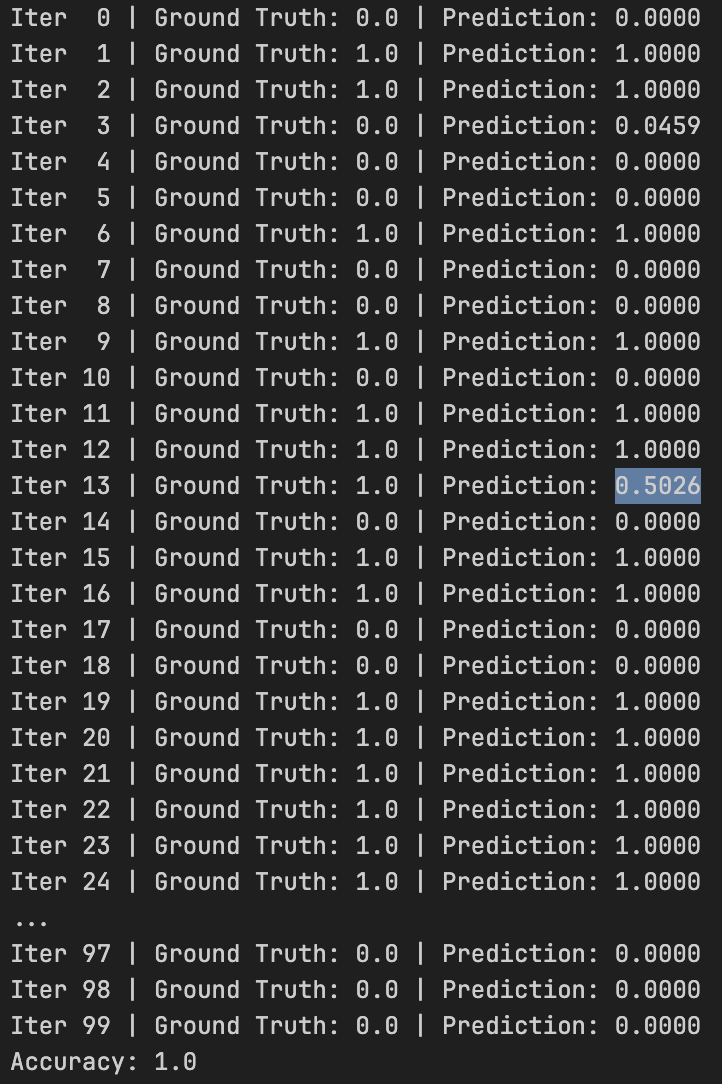
\includegraphics[width=0.7\textwidth]{linear_test.png}
        \caption{Linearly separable data testing prediction}
    \end{subfigure}
    \caption{Linearly separable data results}
\end{figure}

Comparison figure:

\begin{figure}[H]
    \centering
    \centering
    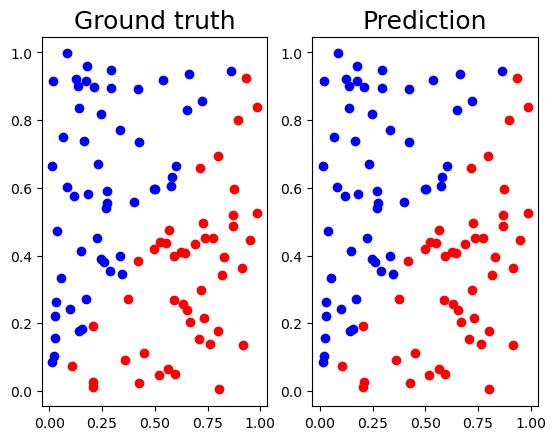
\includegraphics[width=0.5\textwidth]{linear_compare.png}
    \caption{Linearly separable data comparison}
\end{figure}

\subsubsection{XOR data}

Training loss and testing prediction:

\begin{figure}[H]
    \centering
    \begin{subfigure}{0.45\textwidth}
        \centering
        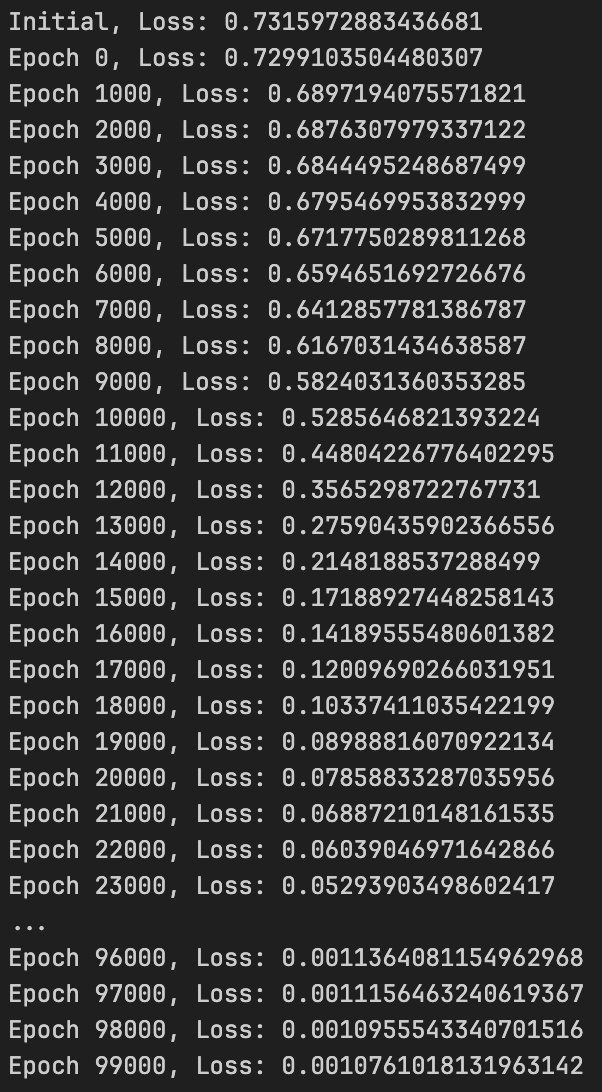
\includegraphics[width=0.6\textwidth]{xor_train.png}
        \caption{XOR data training loss}
    \end{subfigure}
    \begin{subfigure}{0.45\textwidth}
        \centering
        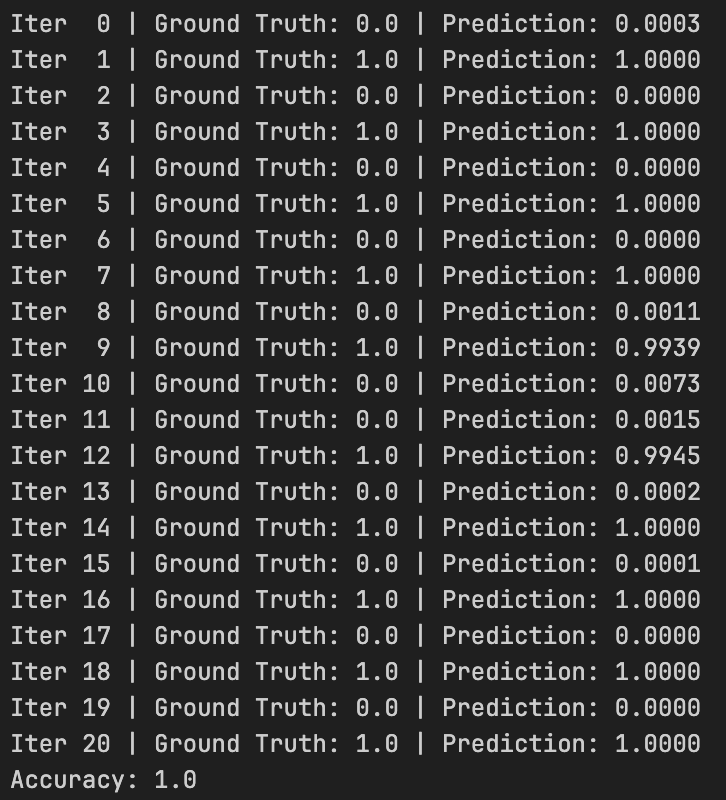
\includegraphics[width=0.9\textwidth]{xor_test.png}
        \caption{XOR data testing prediction}
    \end{subfigure}
    \caption{XOR data results}
\end{figure}

Comparison figure:

\begin{figure}[H]
    \centering
    \centering
    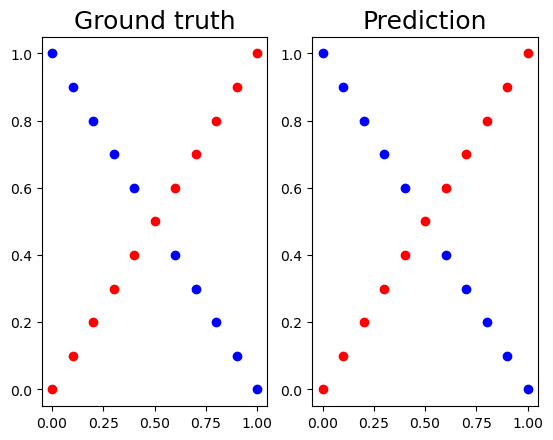
\includegraphics[width=0.5\textwidth]{xor_compare.png}
    \caption{XOR data comparison}
\end{figure}

\subsection{Show the accuracy of your prediction}

The accuracy of the prediction is 100\% for both linearly separable data and XOR data.

\subsection{Learning curve (loss-epoch curve)}

The learning curve of linearly separable data and XOR data is shown below. For linearly separable data, I restricted the epoch shown to 5000.

\begin{figure}[H]
    \centering
    \begin{subfigure}{0.45\textwidth}
        \centering
        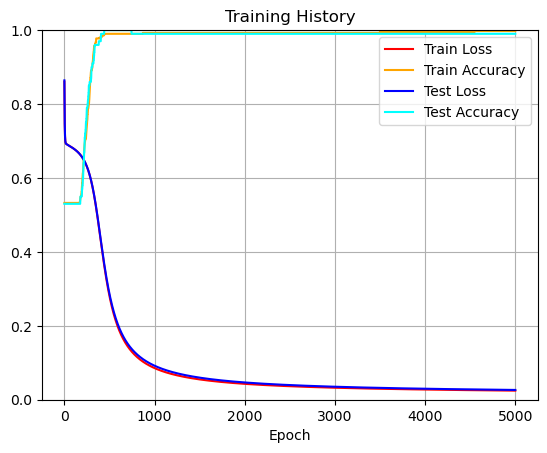
\includegraphics[width=0.8\textwidth]{linear_curve.png}
        \caption{Linearly separable data learning curve}
    \end{subfigure}
    \begin{subfigure}{0.45\textwidth}
        \centering
        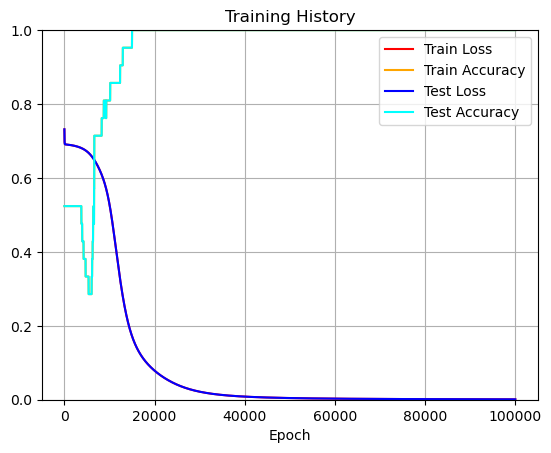
\includegraphics[width=0.8\textwidth]{xor_curve.png}
        \caption{XOR data learning curve}
    \end{subfigure}
    \caption{Learning curve}
\end{figure}

\section{Discussion}

\subsection{Try different learning rates}

I tried different learning rates for linearly separable data .

For lr=100, accuracy achived 100\% in epoch 441

For lr=1, accuracy achived 100\% in epoch 43893, we can observe that it converges very slowly.

lr=5000, accuracy can not achive 100\% in 100000 epochs. The learning curve is shown below. We can observe that the loss oscillates and hard to converge.

\begin{figure}[H]
    \centering
    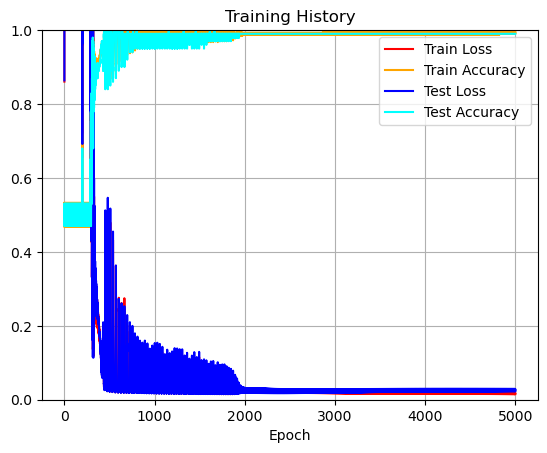
\includegraphics[width=0.5\textwidth]{linear_lr5000.png}
    \caption{lr=5000 learning curve}
\end{figure}

\subsection{Try different numbers of hidden units}

I tried layers [2, 32, 32, 1] for linearly separable data with lr=100. The accuracy is 100\% in epoch 20164, which is much slower than [2, 4, 4, 1].

I also tried layers [2, 1] for linearly separable data with lr=100. The accuracy is 100\% in epoch 989, and the computation needed is much less than [2, 4, 4, 1]. So it can be trained faster with fewer hidden units.

\subsection{Try without activation functions}

Without activation functions, the model is often encountered with the vanishing gradient problem, which makes me need to add a small value in the gradient calculation to avoid division by zero.

The model without activation functions is more unstable and harder to converge in the linearly separable data. The learning curve is shown below.

\begin{figure}[H]
    \centering
    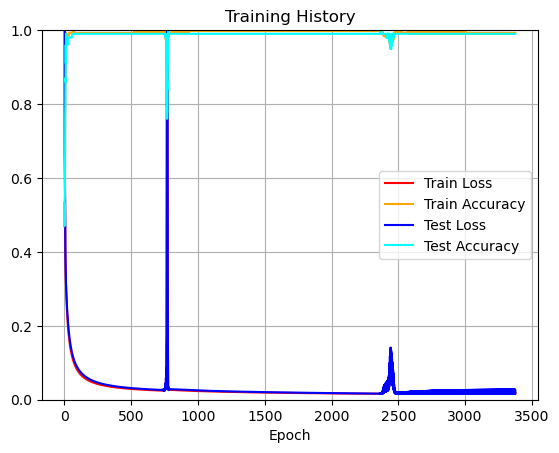
\includegraphics[width=0.5\textwidth]{linear_no_activation_curve.png}
    \caption{No activation function learning curve}
\end{figure}

The model without activation functions can not learn the XOR data. It always predicts the same label as shown below.

\begin{figure}[H]
    \centering
    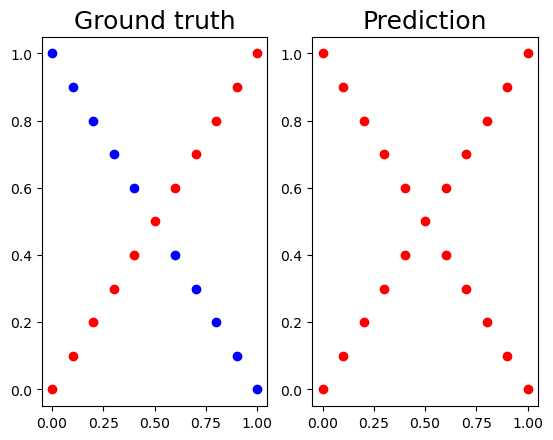
\includegraphics[width=0.5\textwidth]{xor_no_activation.png}
    \caption{No activation function XOR data prediction}
\end{figure}

\section{Question}

\subsection{What is the purpose of activation functions?}

Activation functions, such as ReLU or sigmoid, are used to introduce non-linearity to the neural network. Without activation functions, the neural network would be a linear model, and it would not be able to learn complex patterns in the data, such as XOR data.

\subsection{What might happen if the learning rate is too large or too small?}

When the learning rate is too large, the model may not converge, and the loss may oscillate or even diverge. When the learning rate is too small, the model may converge very slowly, and it may get stuck in a local minimum.

\subsection{What is the purpose of weights and biases in a neural network?}

Weights and biases are the parameters of the neural network.

Weights are used to multiply the input features/activations to get the output of each layer, determining the importance of each feature/activation.

Biases are used to shift the output of each layer, allowing the model to determine the threshold of the activation.

The weights and biases are learned during the training process to minimize the loss function.

\section{Extra}

\subsection{Implement different optimizers.}

I implemented the \bfr{Adam} optimizer in the model. For lr=1, beta1=0.9, beta2=0.999, epsilon=1e-8, the model can achieve 100\% accuracy in epoch 199 on linearly separable data, which is faster than the default optimizer.

The learning curve is shown below:

\begin{figure}[H]
    \centering
    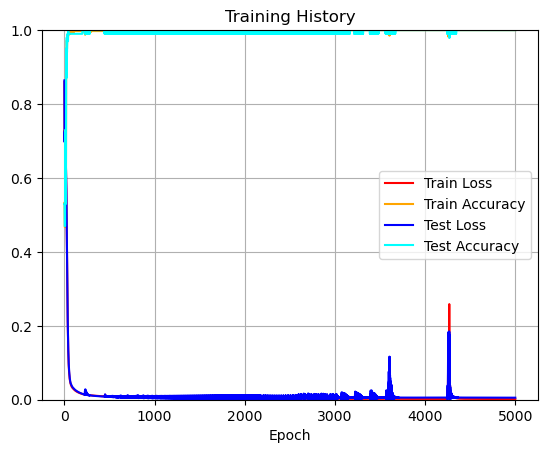
\includegraphics[width=0.5\textwidth]{linear_adam_curve.png}
    \caption{Adam optimizer learning curve}
\end{figure}

\subsection{Implement different activation functions.}

I implemented the \bfr{ReLU} activation function in the model. The model can still achive 99\% accuracy, with much faster convergence compare to sigmoid. but the consistency is not as good as sigmoid.

The learning curve is shown below:

\begin{figure}[H]
    \centering
    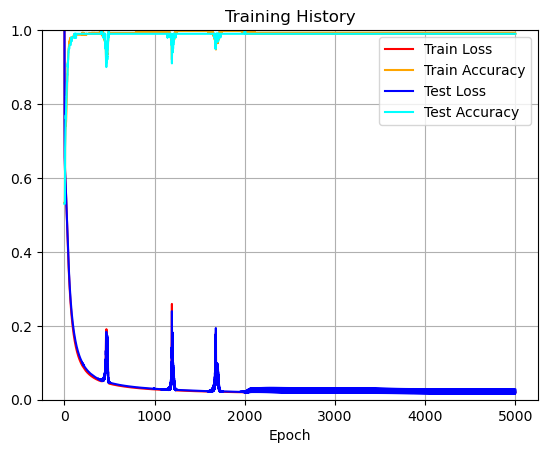
\includegraphics[width=0.5\textwidth]{linear_relu_curve.png}
    \caption{ReLU activation function learning curve}
\end{figure}

\end{document}